The stability of the ten photodiodes used to survey the \laser~light is monitored with a LED signal. The light is also transmitted to a reference photodiode for normalization. The reference photodiode is monitored with a radioactive source.\\
A view of the \phocal~box is given on figure \ref{fig:lasphocal}. The main components are:
\begin{itemize}
\item LED box: houses the LED (Nichia blue NSPB520S $\lambda$=470 nm \cite{ref:led}) itself and a LED driver that provides a pulsed signal lasting 10 ns with an intensity that may be tweaked manually thanks to a potentiometer between 1 and 20 V.
\item reference box: the reference photodiode (Hamamatsu S2744 \cite{ref:bigphoto}, active area: 10x20 mm$^2$, peak sensitivity wavelength: 960 nm) is located in this box. It receives the LED signal through an optics fiber connected to the LED box. The stability of this photodiode is monitored with a radioactive $\alpha$-source of $^{241}$Am (activity: 3.7 kBq, T$_{1/2}$=432.2 y, E$_{\alpha}$=5.486 MeV) placed in front of it. Because of their charge and large mass, alpha particles can travel only a few centimetres in air. To maximize the radioactive signal dry air is injected in front of the reference photodiode.
\item Logic board: this card is used to drive the \phocal~system. It provides a 90 Hz signal to trigger the LED signal. This frequency has been chosen so as to keep the coïncidence rate of the radioactive source and the LED signals at the sub-percent level.
\item optics fibers and light mixers: the LED signal is transmitted to optics fibers (plastic fibers with a core diameter of 908 $\mu$m \cite{ref:fibers}) through epoxy pieces embedded in PMMA blocks.
\end{itemize}
Two temperature (one in the reference box, the other in the LED box) and one humidity (in the reference box) probes are used to measure the environmental conditions in the \phocal~box. 

\begin{figure}[htbp]
\centering
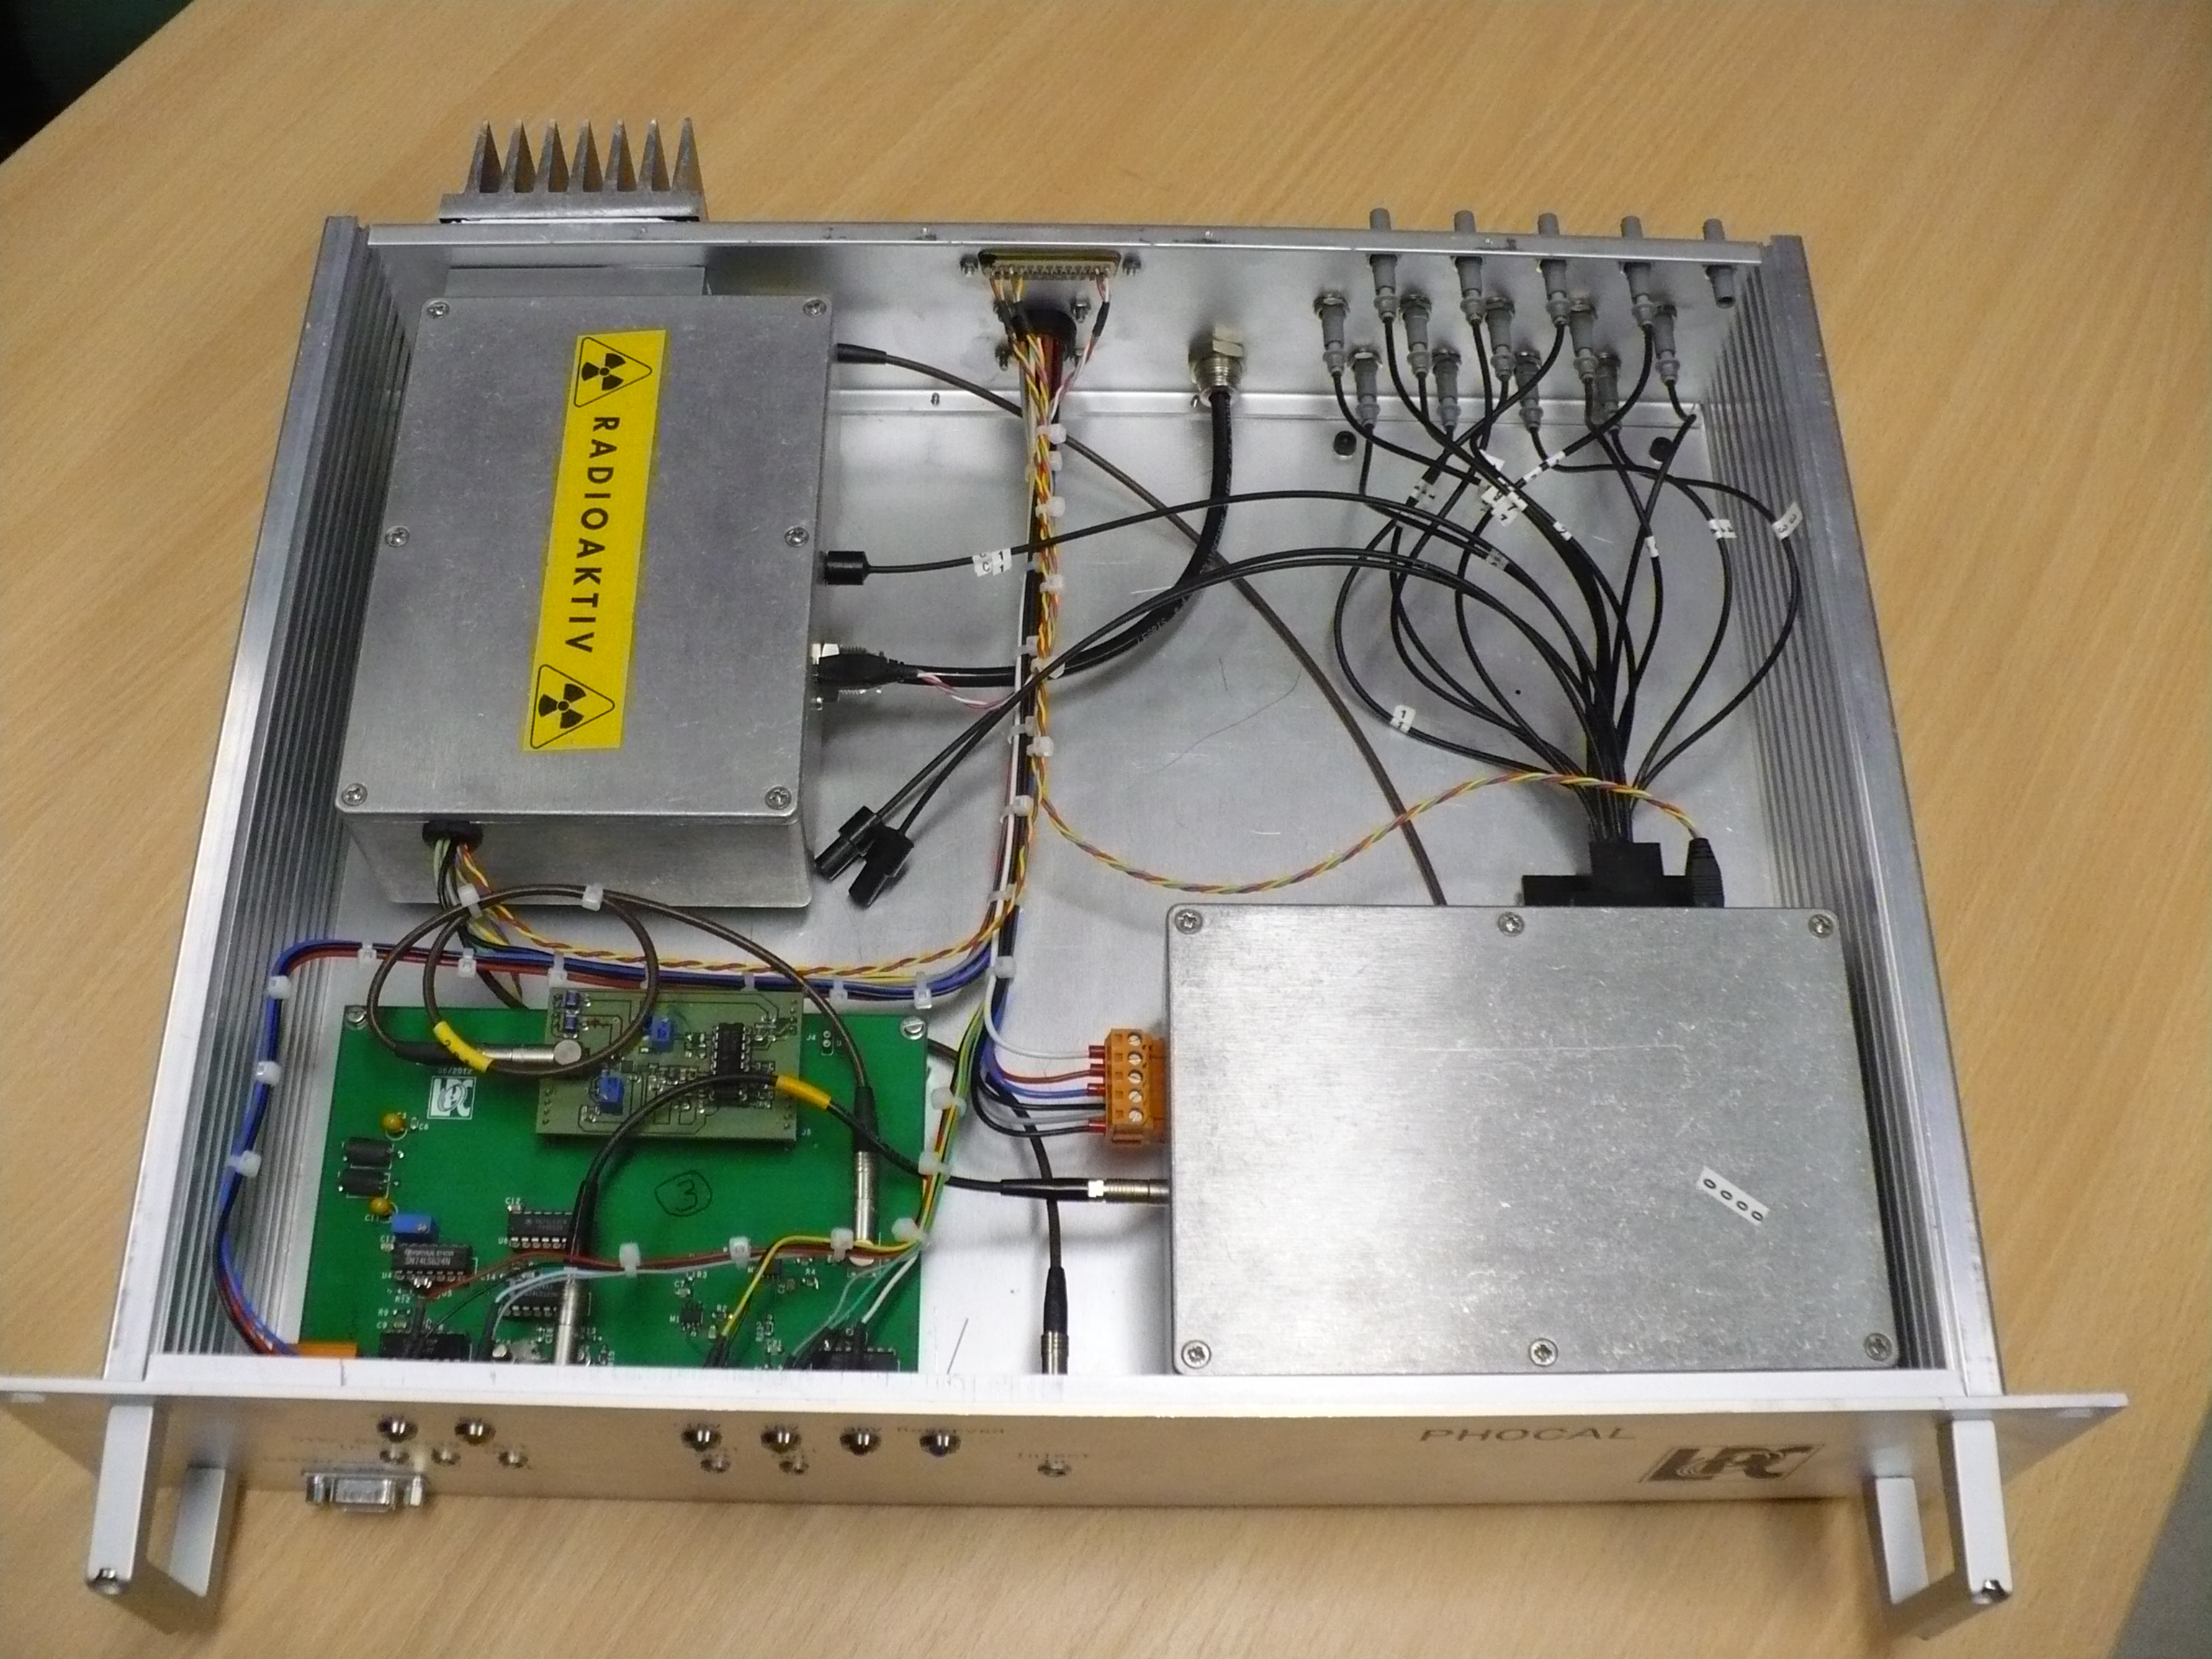
\includegraphics[height=6cm]{figures/phocal1.JPG}
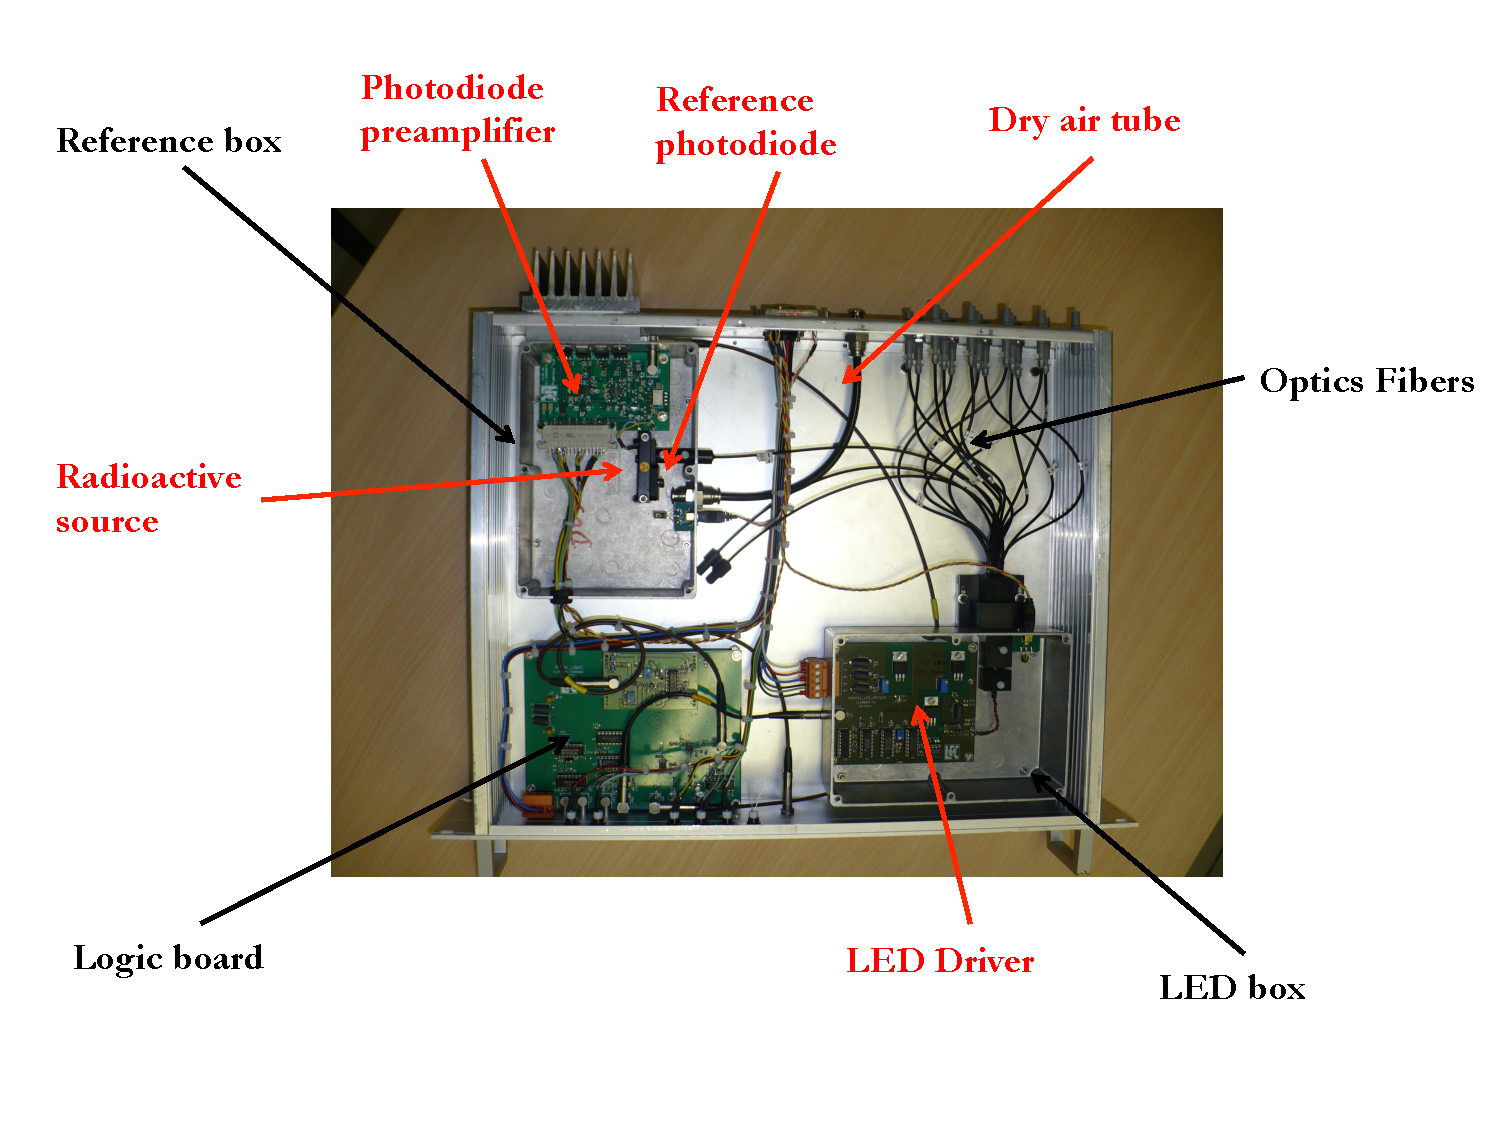
\includegraphics[height=10cm]{figures/phocal2_comm.pdf}
\caption{Views of the \phocal~system}\label{fig:lasphocal}
\end{figure}